\documentclass[11pt, oneside]{article} 	% use "amsart" instead of "article" for AMSLaTeX format
\usepackage{geometry} 		% See geometry.pdf to learn the layout options. There are lots.
\geometry{letterpaper} 		% ... or a4paper or a5paper or ... 
\usepackage[parfill]{parskip} 		% Activate to begin paragraphs with an empty line rather than an indent
\usepackage{graphicx}				% Use pdf, png, jpg, or eps§ with pdflatex; use eps in DVI mode
								% TeX will automatically convert eps --> pdf in pdflatex		
\usepackage{amssymb}
\usepackage{amsmath}
\usepackage{authblk}
\usepackage{framed}
\usepackage[
backend=biber,
style=alphabetic,
]{biblatex}
\usepackage{graphicx}
\graphicspath{ {./images/} }
\usepackage{verbatim}
\usepackage{tikz} 
\usepackage{xcolor,colortbl}
\usepackage{subcaption}
\captionsetup{compatibility=false}
\usepackage{syntonly}


\title{Spotting Graph Theory Problems in Spot It}
\author[1]{Dave Fetterman}
\author[2]{James Wang}
\affil[1]{Obviously Unemployed}
\affil[2]{Surprisingly Employed}

\date{4/13/23}
\begin{document}
\maketitle

\begin{abstract}

The card game ``Spot It'' supports a unique mechanic: every card of the deck has eight different symbols, and shares exactly one symbol of some kind with every other card.  The obvious game play (``spot the match') works for children as young as two; the intricacies of deck construction astound these children of forty-two. In hypothetically constructing our own deck, we run across interesting problems in graph theory, number theory, and abstract algebra.  Some are solved, some remain unsolved.  Until now.  Not really.  We just prove hard things are hard.
\\

Notably, starting with $g=p^k, p \in \mathbb{P}, k \in \mathbb{N}$ and $n = g^2+g+1$, we prove the following four constructions are equivalent:
\\
\begin{enumerate}
\item (The Children's Game) A deck of $n$ ``Spot It'' Cards with $s=g+1$ symbol slots, where each of $m = n$ symbols occurs exactly $g+1$ times,
\item (Graph Theory) An edge partition of the complete graph $K_n$ into complete subgraphs $K_g$,
\item (Abstract Algebra) A finite (Galois) field of order $g$, and
\item (Number Theory) A Perfect Difference Set\cite{1} on $n$ elements.
\end{enumerate} 
   
We then examine other configurations of $s$ and $g$, as well as comment on other reasonable constructions of a Spot It Card deck.

\end{abstract}

\section{The game and the problem}

Introduced to us by Ari Steinberg, ``Spot It'' is a children's game of 55 cards as shown in Figure~\ref{fig:cards}, featuring eight colorful symbols on each.  Though gameplay comes with a few variants in its tiny rulebook, the primary mechanic when presented two cards is simply \emph{spot single the common symbol first}. The game is simple enough for a two- or three-year old to grasp (and win!), but this poses the question: \emph{just how did they construct such a deck?} 

\emph{Note: There have been some other investigations here\cite{2}, but for the purposes of enjoyment, everything in this paper was researched without reference to prior (Spot It) work.}


\begin{figure}[!htb]
\centering
\begin{subfigure}{.2\textwidth}
 \centering
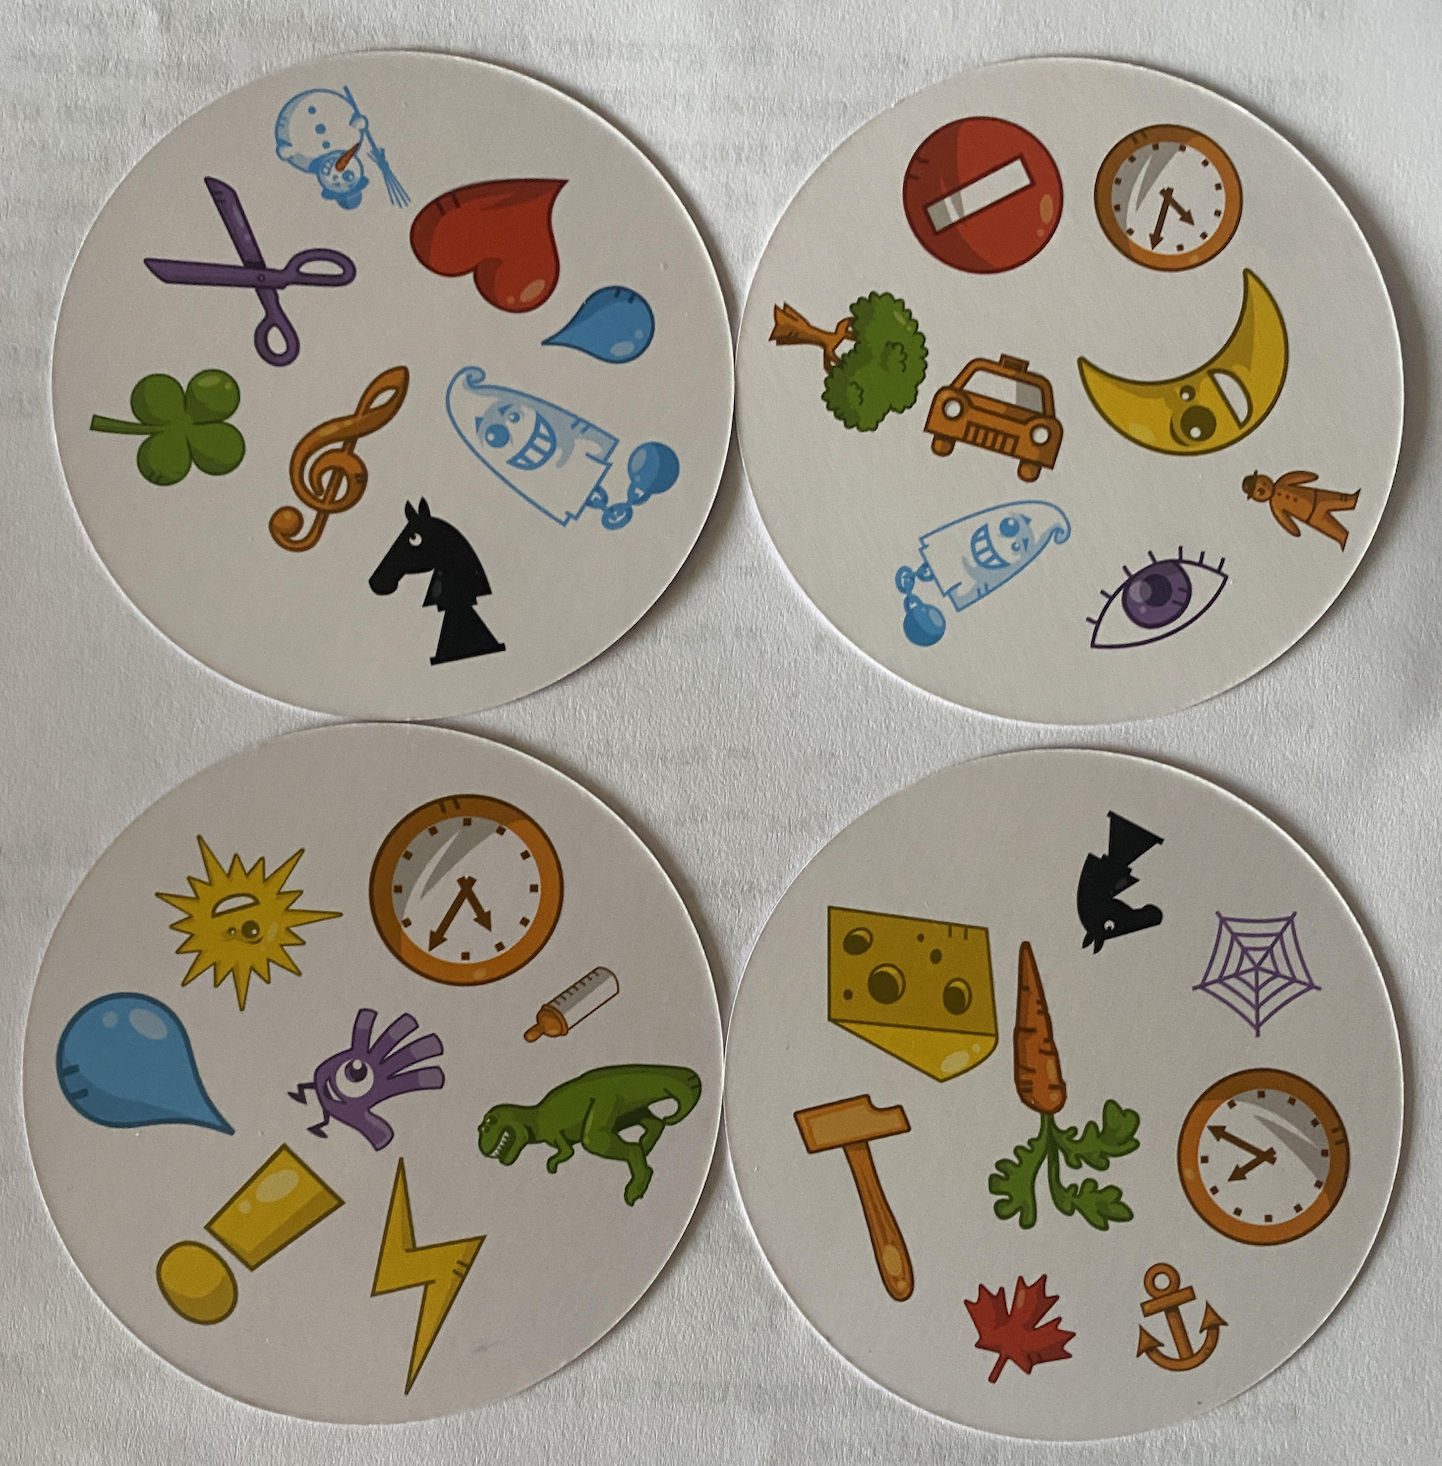
\includegraphics[scale=.2]{cards}
\caption{Four cards in the game}
\label{fig:cards}
\end{subfigure}

\begin{subfigure}{.2\textwidth}
 \centering
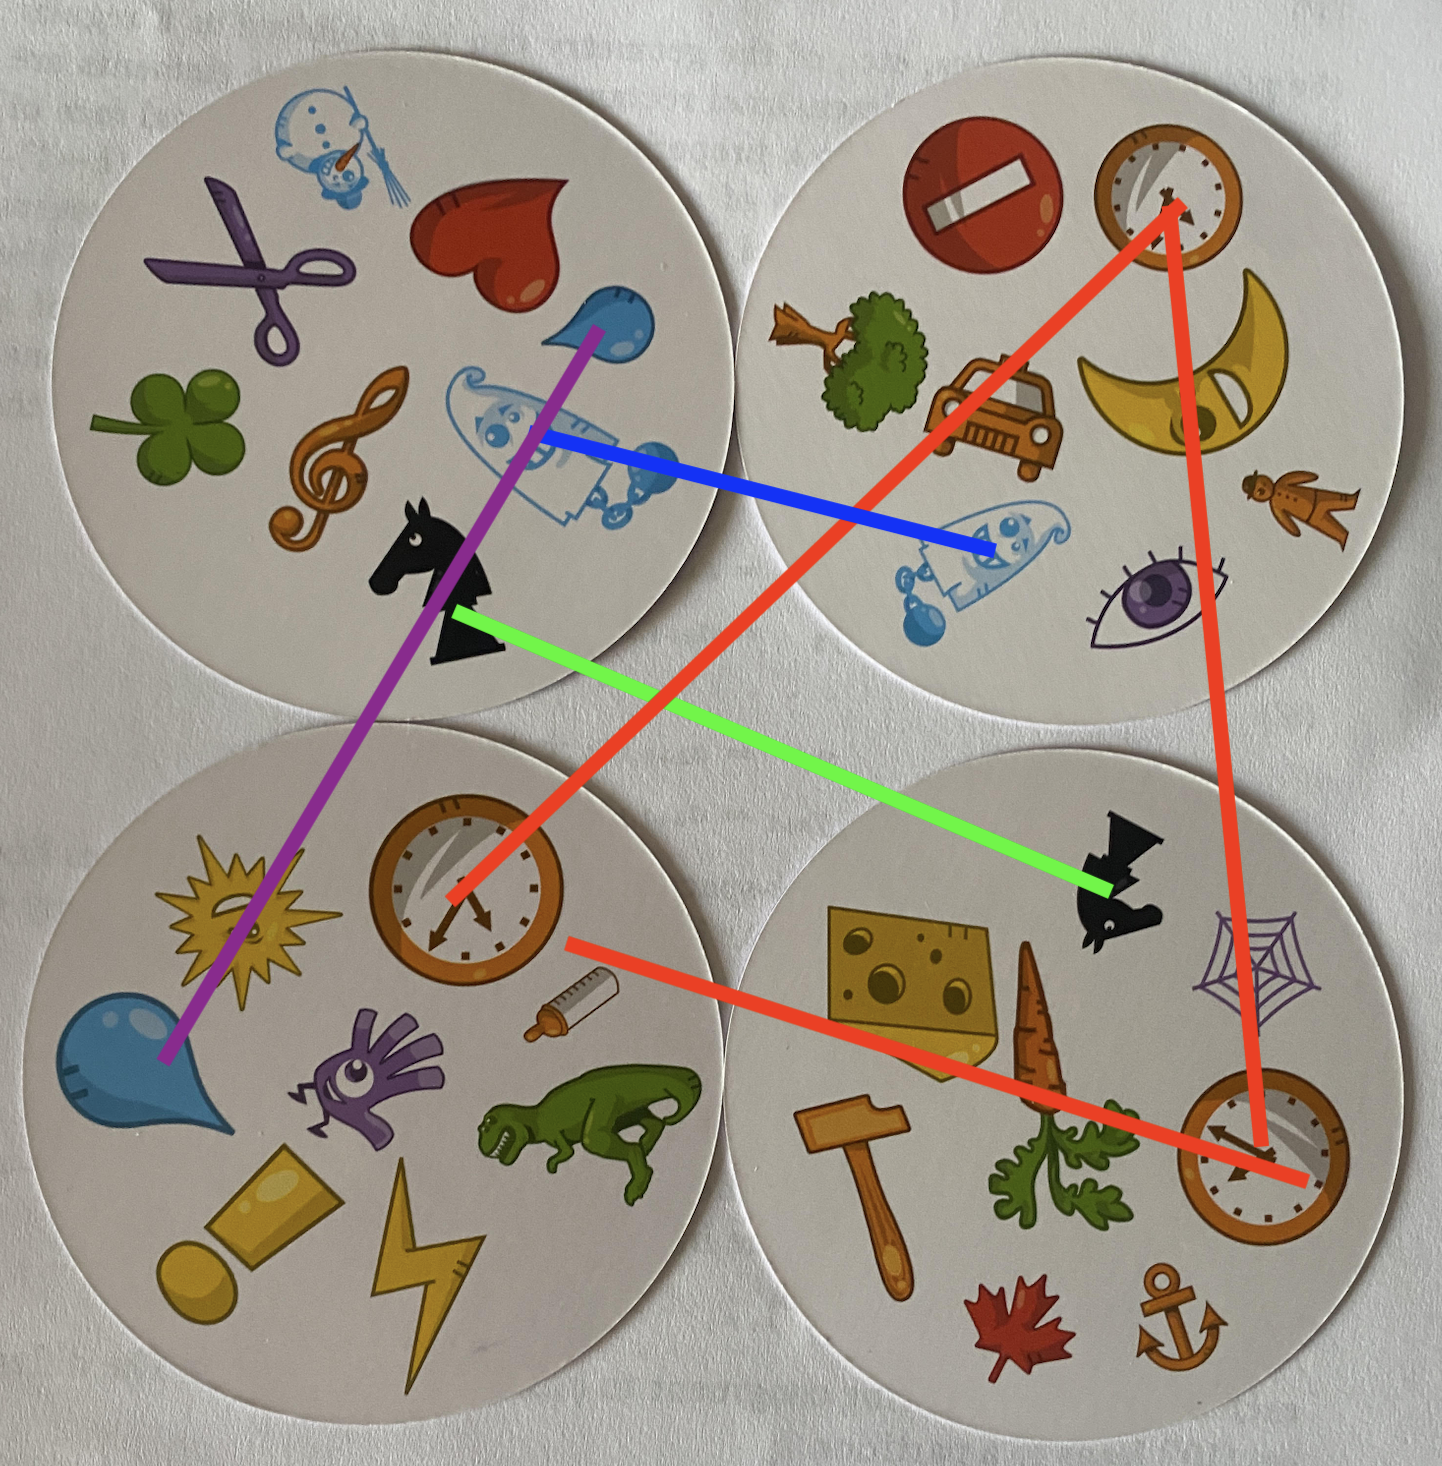
\includegraphics[scale=.2]{cards-links}
\caption{Four cards in the game with links}
\label{fig:cards-links}
\end{subfigure}

\begin{subfigure}{.2\textwidth}
\centering
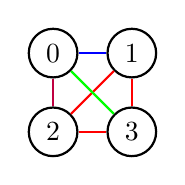
\begin{tikzpicture}
\begin{scope}[every node/.style={circle,thick,draw}]
\node (0) at (0, 1)  {0}; 
\node (1) at (1, 1) {1}; 
\node (2) at  (0, 0) {2}; 
\node (3) at  (1, 0) {3}; 

\draw[thick, red] (1) -- (2); 
\draw[thick, red] (1) -- (3); 
\draw[thick, red] (2) -- (3); 

\draw[thick, blue] (0) -- (1); 
\draw[thick, green] (0) -- (3); 
\draw[thick, purple] (0) -- (2); 
\end{scope}
\end{tikzpicture}
\caption{Four cards graph}
\label{fig:cards-graph}
\end{subfigure}

\end{figure}

Naturally, there are trivial constructions: every symbol occurs only twice, or once, or the count of symbols is so varied that a deck can be constructed almost greedily.  However, the Spot It game has uniformly 8 symbol ``slots'' on each card, which each appear 8 times \footnote{As we will see later, there should be 57 cards for this to be true; it's likely two cards were removed} across the different cards.  

This is what we examine in this paper:

\begin{framed}
\textbf{The Core Question:} For what choices of $g$ and $s$ can we construct a ``Spot It'' deck where each of the $s$ symbols on each card appears exactly $g$ times throughout the deck?
\end{framed}

\subsection{Reframing as a graph}
Noticing that every card has a relationship to every other card (notably, the identity of the single symbol shared between them) as in Fig.~\ref{fig:cards-links}, we take our first step by reconstructing this problem as an undirected graph as in Fig.~\ref{fig:cards-graph}. 


\begin{figure}[!htb]
\centering
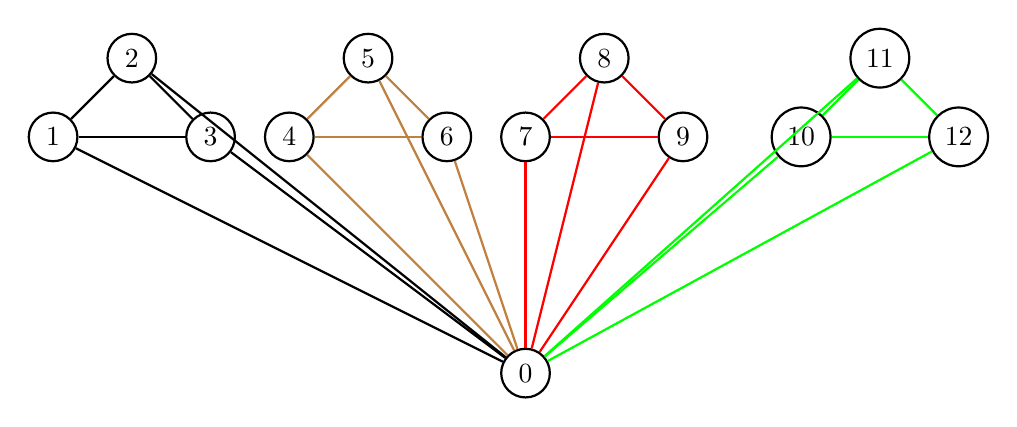
\begin{tikzpicture}
\begin{scope}[every node/.style={circle,thick,draw}]
\node (0) at (0, -2)  {0}; 
\node (1) at (-6, 1) {1}; 
\node (2) at  (-5, 2) {2}; 
\node (3) at  (-4, 1) {3}; 
\node (4) at (-3, 1) {4}; 
\node (5) at  (-2, 2) {5}; 
\node (6) at  (-1, 1) {6}; 

\node (12) at (5.5, 1) {12}; 
\node (11) at  (4.5, 2) {11}; 
\node (10) at  (3.5, 1) {10}; 
\node (9) at (2, 1) {9}; 
\node (8) at  (1, 2) {8}; 
\node (7) at  (0, 1) {7}; 

\draw[thick, black] (0) -- (1); 
\draw[thick, black] (0) -- (2); 
\draw[thick, black] (0) -- (3);  

\draw[thick, black] (2) -- (3); 
\draw[thick, black] (1) -- (2); 
\draw[thick, black] (1) -- (3);  


\draw[thick, brown] (0) -- (4); 
\draw[thick, brown] (0) -- (5); 
\draw[thick, brown] (0) -- (6);  

\draw[thick, brown] (5) -- (6); 
\draw[thick, brown] (4) -- (5); 
\draw[thick, brown] (4) -- (6);  


\draw[thick, red] (0) -- (7); 
\draw[thick, red] (0) -- (8); 
\draw[thick, red] (0) -- (9);  


\draw[thick, red] (8) -- (9); 
\draw[thick, red] (7) -- (8); 
\draw[thick, red] (7) -- (9);  


\draw[thick, green] (0) -- (10); 
\draw[thick, green] (0) -- (11); 
\draw[thick, green] (0) -- (12);  


\draw[thick, green] (11) -- (12); 
\draw[thick, green] (10) -- (11); 
\draw[thick, green] (10) -- (12);  

\end{scope}
\end{tikzpicture}
\caption{$n = s(g-1)+1$.  Here, $s=4, g=3$}
\label{fig:graph-theorem}
\end{figure}


\begin{framed}
\textbf{The Graph Representation:} A deck of Spot It Cards each with $s$ symbol slots, where each symbol appears $g$ times c can be represented by a graph $G$:
\begin{enumerate}
\item With $n$ nodes, where $n = s(g-1) + 1$
\item With $m$ unique edge colors, where $m$ denotes the number of symbols,
\item Where all edges of color $m_i$ form a complete subgraph on $g$ nodes, s, and $m = {n \choose 2} / {g \choose 2}$.
\end{enumerate}
\end{framed}

\emph{Note: Singletons (groups where $g=1$) would be rendered as self-edges.  These are uninteresting and are generally ignored in this paper}

\emph{Proof}:
\begin{enumerate}
\item As in Fig.~\ref{fig:graph-theorem}, node $n_0$'s adjacencies are exactly $s$ monocolor cliques of size $g-1$ (excluding $n_0$ itself).  In a complete graph, these adjacencies comprise the total node set, so $n = (g-1)s + 1$ when adding $n_0$ back in.  Using any other node is equivalent.
\item As in Fig.~\ref{fig:cards-links}, while card 1 and card 2 having the relationship ``clock'', node 1 and node 2 instead share an edge with the color red.  This is the same relationship between nodes 2 and 3, and nodes 1 and 3.  ``Drop'', ``knight'', and ``ghost'' would be colors purple, green, and blue, respectively.  This works because every edge has exactly one color (corresponding 1:1 with a symbol) in this formulation, and every card pair has exactly one symbol shared.
\item All cards with a given symbol (say, ``clock'') must correspond to nodes be linked with the color red to all other nodes whose card has a clock; this is a complete subgraph.  A complete graph $K_n$ has ${n \choose 2}$ edges.  A monocolor clique of size $g$ is a complete graph as well, with ${g \choose 2}$ edges.  $K_n$'s edges are exactly these equal-sized cliques, so there are therefore $m = \frac{{n \choose 2}}{{g \choose 2}}$ of them, corresponding to colors.
\end{enumerate}

And since every edge in our complete graph $K_n$ is in exactly one monocolor clique of size $K_g$, this becomes a crisp graph theory problem.

\begin{framed}
\textbf{The Core Question in Graph Terms}: Given $s$ and $g$ as before, can we construct an edge partition (colloquially here, ``coloring'')\footnote{Our idiosyncratic ``coloring'' should not be confused with the traditional ``edge coloring'', where no edges of the same color can meet at a node} of $K_n$ into a set of complete subgraphs of size g (denoted $K_g$)?
\end{framed}
% TODO why isn't the footnote showing?
\textbf{Though exhaustive research wasn't done, this graph problem does not appear to have a clear analytical solution out there.}\footnote{Or people who care about publishing it within the reach of lazy hobbyists, anyway!}

Since $m$ and $n$ are determined from $s$ and $g$, we'll start by looking at possibly candidate configurations of $s$ and $g$.

\section{The Candidate Theorem: $g | s(s-1), g \leq s$}

Suppose that that every symbol $s$ has exactly $g$ cards containing it \footnote{for example, all $s=7$ symbols in Fig.~\ref{fig:s7g3} correspond to cliques of size $g=3$}.  Then 

\begin{framed}
\begin{enumerate}
\item $g | s(s-1)$.
\item If $s >1 $ and $g > 1$ then $g \leq s$ 
\item Corollary to (2): $m = (\frac{s}{g})n$ and therefore $m \geq n$
\item All candidate configurations of $g, s$ are $g \leq s$, $g | s(s-1)$.
\end{enumerate}
\end{framed}

\emph{Proof}:
\begin{enumerate}
\item 
\begin{align}
{g \choose 2} \bigg| {n \choose 2} \Rightarrow \frac{n(n-1)}{g(g-1)} \in \mathbb{N} \Rightarrow g(g-1) | n(n-1) \\
 n = (g-1)s+1 \Rightarrow g(g-1) \big| (sg-s+1)(sg-s) = (sg-s+1)s(g-1)\\
\Rightarrow g | s^2g - s^2 + s \Rightarrow g | (1-s)s \Rightarrow g | s(s-1) 
\end{align}
\item Any node $n_i$ is adjacent to $s$ monocolor cliques of size $g$.  These cliques $C_1 ... C_s$, containing non-$n_i$ nodes if $g > 1$, comprise all nodes, and any other cliques can contain no more than one of each $K_i$.  This means that clique of size $g$ greater than $s$ cannot be formed, since the only place to find nodes are these $C_1 ... C_s$.  The other trivial case, $s=1$, means there is only one color in the whole graph. 
\\
This means we need not consider configurations like $g = 6, s=3$ even though $6 | 3(3-1)$.

\item Another corollary here is that \fbox{$m \geq n$}, since:
\begin{align}
n = (sg - s + 1) \\
m = \frac{{(sg - s + 1)(sg-s) \choose 2}}{{g \choose 2}} = \frac{(sg-s+1)(sg-s)}{g(g-1)} = \frac{(sg-s+1)s}{g} \\
\Rightarrow m = (\frac{s}{g})n\\
s \geq g \Rightarrow m \geq n
\end{align}
\item This is just a combination of (1) and (2).  But for example, a tiling of triangles ($g=3$) means that either $s \equiv 0 \mod 3$ (see Fig.~\ref{fig:s3g3})
 or $s \equiv 1 \mod 3$ (see Fig, ~\ref{fig:s4g3}).  
\end{enumerate}




\begin{figure}[!htb]
\centering
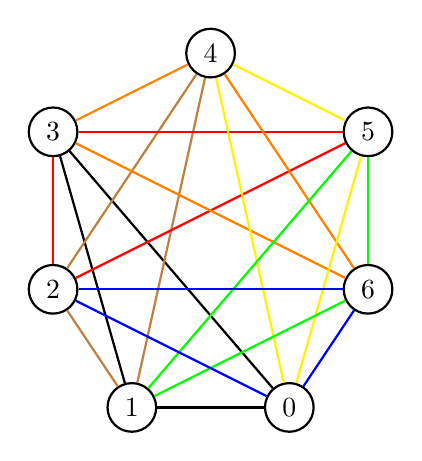
\begin{tikzpicture}
\begin{scope}[every node/.style={circle,thick,draw}]
  \node (0) at (3,0.5) {0};
  \node (1) at (1,0.5) {1};
  \node (2) at (0,2) {2};
  \node (3) at (0,4) {3};
  \node (4) at (2,5) {4};
  \node (5) at (4,4) {5};
  \node (6) at (4,2) {6};
  
  
\draw[thick, black] (0) -- (1); 
\draw[thick, black] (1) -- (3); 
\draw[thick, black] (0) -- (3); 

\draw[thick, brown] (1) -- (2); 
\draw[thick, brown] (2) -- (4); 
\draw[thick, brown] (1) -- (4); 

\draw[thick, red] (2) -- (3); 
\draw[thick, red] (3) -- (5); 
\draw[thick, red] (2) -- (5); 

\draw[thick, orange] (3) -- (4); 
\draw[thick, orange] (4) -- (6); 
\draw[thick, orange] (3) -- (6); 

\draw[thick, yellow] (4) -- (5); 
\draw[thick, yellow] (5) -- (0); 
\draw[thick, yellow] (4) -- (0); 

\draw[thick, green] (5) -- (6); 
\draw[thick, green] (6) -- (1); 
\draw[thick, green] (5) -- (1); 

\draw[thick, blue] (6) -- (0); 
\draw[thick, blue] (0) -- (2); 
\draw[thick, blue] (6) -- (2); 


\end{scope}
\end{tikzpicture}
\label{fig:s3g3}
\caption{s=3, g=3, n=7, m=7.  Cliques of form $(n_i, n_{i+1}, n_{i+3})$. for all $i$}
\end{figure}




\begin{figure}[!htb]
\centering
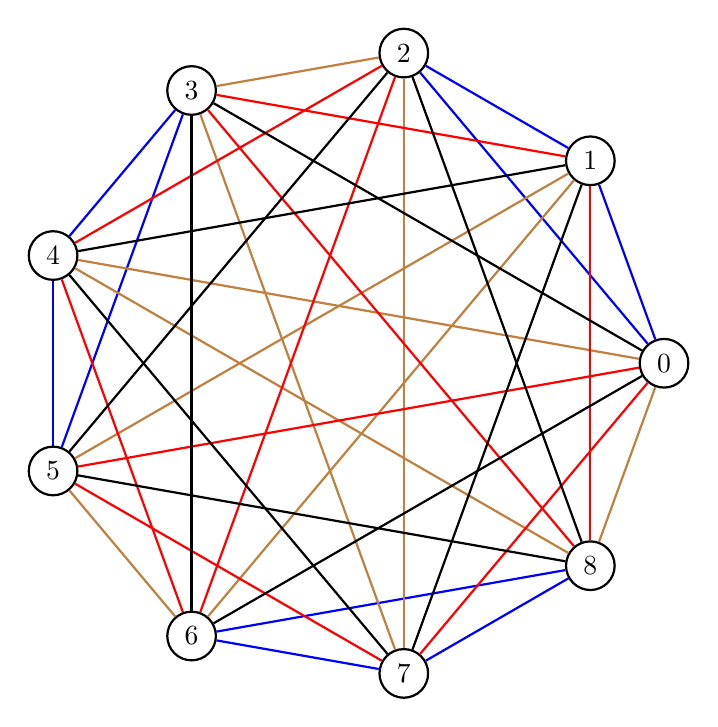
\begin{tikzpicture}
\begin{scope}[every node/.style={circle,thick,draw}]

\node (0) at (4,0) {0};
\node (1) at (3.064,2.571) {1};
\node (2) at (0.695,3.939) {2};
\node (3) at (-2,3.464) {3};
\node (4) at (-3.759,1.368) {4};
\node (5) at (-3.759,-1.368) {5};
\node (6) at (-2,-3.464) {6};
\node (7) at (0.695,-3.939) {7};
\node (8) at (3.064,-2.571) {8};
  
\draw[thick, blue] (0) -- (1); 
\draw[thick, blue] (1) -- (2); 
\draw[thick, blue] (0) -- (2); 

\draw[thick, blue] (3) -- (4); 
\draw[thick, blue] (4) -- (5); 
\draw[thick, blue] (3) -- (5); 

\draw[thick, blue] (6) -- (7); 
\draw[thick, blue] (7) -- (8); 
\draw[thick, blue] (6) -- (8); 

\draw[thick, brown] (0) -- (4); 
\draw[thick, brown] (0) -- (8); 
\draw[thick, brown] (4) -- (8); 

\draw[thick, brown] (3) -- (7); 
\draw[thick, brown] (3) -- (2); 
\draw[thick, brown] (7) -- (2); 

\draw[thick, brown] (6) -- (1); 
\draw[thick, brown] (6) -- (5); 
\draw[thick, brown] (1) -- (5); 

\draw[thick, red] (0) -- (5); 
\draw[thick, red] (0) -- (7); 
\draw[thick, red] (5) -- (7); 

\draw[thick, red] (3) -- (8); 
\draw[thick, red] (3) -- (1); 
\draw[thick, red] (8) -- (1); 

\draw[thick, red] (6) -- (2); 
\draw[thick, red] (6) -- (4); 
\draw[thick, red] (2) -- (4); 


\draw[thick, black] (0) -- (3); 
\draw[thick, black] (0) -- (6); 
\draw[thick, black] (3) -- (6); 

\draw[thick, black] (1) -- (4); 
\draw[thick, black] (1) -- (7); 
\draw[thick, black] (4) -- (7); 

\draw[thick, black] (2) -- (5); 
\draw[thick, black] (2) -- (8); 
\draw[thick, black] (5) -- (8); 


\end{scope}



\end{tikzpicture}
\label{fig:s4g3}
\caption{s=4, g=3, n=9, m=12.  \\
Cliques: $(n_i, n_{i+3}, n_{i+6}), (n_i, n_{i+1}, n_{i+2}), (n_i, n_{i+4}, n_{i+8}), (n_i, n_{i+5}, n_{i+7}), 3 | i $}
\end{figure}



\section{Constructing $g = s-1$ over a field}

Though we presented a few legitimate examples of complete graphs tiled by uniformly sized complete subgraphs in Fig.~\ref{fig:s3g3} and Fig.~\ref{fig:s4g3}, these are not easy to find by hand once $s$ becomes much larger.  The whole problem of graph partitioning admits many algorithms, most approximations\cite{3}, though usually over an arbitrary graph instead of a relatively simple complete graph, and many referring to separating actual \emph{nodes} into partitions, rather than edges.

We can, however, systematically find an edge partition if $g$ is a prime power.

\begin{framed}
\textbf{g=s-1 construction}: If $g$ is a prime power $p^k$, we can explicitly construct a graph that satisfies our game with $g = s-1$.
\end{framed}


As the combination of $s, g$ determine the shape of the graph entirely, $g = s-1$ implies:
\begin{itemize}
\item The graph has $n = s(g-1) + 1 = (g+1)(g-1) + 1 = g^2$ nodes.
\item Those nodes can be grouped into $g$ groups of size $g$.
\item There are $m = (\frac{s}{g}) n = (\frac{s}{g}) g ^2 = sg = (g+1)g$ colors in the graph.
\end{itemize}


We can start with the easiest way to see this: $g = p, p \in \mathbb{P}$.

Construct the multiplication table for the finite field on $p=3$, as in Fig. ~\ref{fig:gf3-tables}.


\begin{figure}[!htb]
\centering
\begin{subfigure}{.3\textwidth}
 \centering
 \begin{tabular}{c | c c c}
      + & 0 & 1 & 2 \\
\hline
     0 & 0 & 1 & 2 \\
     1 & 1 & 2 & 0 \\
     2 & 2 & 1 & 0 \\
     \end{tabular}
 \caption{Addition table GF(3)}
\label{fig:gf3-add}
\end{subfigure}
\begin{subfigure}{.3\textwidth}
 \centering
\begin{tabular}{c | c c c}
     $\cdot$ & 0 & 1 & 2 \\
\hline
     0 & 0 & 0 & 0  \\
     1 & 0 & 1 & 2  \\
     2 & 0 & 2 & 1  \\

\end{tabular}
\caption{Multiplication table GF(3)}
\label{fig:gf3-mult}
\end{subfigure}
\caption{Field tables for GF(3)}
\label{fig:gf3-tables}
\end{figure}

\begin{framed}
To construct the $m = g(g-1)$ colors (symbol cliques) in the graph:
\begin{itemize}
  \item Construct a finite field $\mathcal{GF(g)}$, which is of size $g$.
  \item Divide the $g^2$ nodes into $g$ groups $(G_0, G_1, G_2 ... G_{g-1})$, where $[0...g-1] \in \mathcal{F}$, of $g$ nodes each $((G_{0,0}, G_{0,1}...G_{0,g-1}) ...G_{g-1,0}, G_{g-1,1}...G_{g-1,g-1})$
  \item For all $c \in [0,g-1]$: 
  \begin{itemize}
    \item For all $y \in [0,g-1]$:   
    \begin{itemize}
       \item Set $C_{c,y}$ to the empty set.
       \item For all $x \in [0,g-1]$, add $G_{x, G_x \cdot G_y + c}$ to clique $C_{c, y}$, where $+$ and $\cdot$ refer to addition and multiplication rules for $\mathcal{F}$.
     \end{itemize}
  \end{itemize}
  \item The $g$  cliques formed from the node groups  $(G_0, G_1, G_2 ... G_{g-1})$, plus the $g^2$ cliques like $C_c, y$ form the $(g+1)g$ cliques or ``colors''.
\end{itemize}
\end{framed}




\begin{figure}[!htb]
\centering
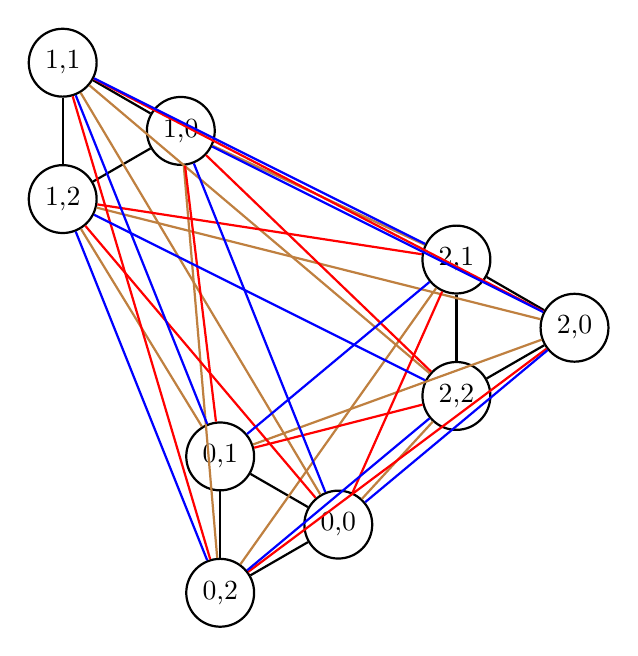
\begin{tikzpicture}
\begin{scope}[every node/.style={circle,thick,draw}]
\node (0) at (1,0)  {0,0}; 
\node (1) at (-.5, .866) {0,1}; 
\node (2) at  (-.5, -.866) {0,2}; 

\node (3) at (-1,5)  {1,0}; 
\node (4) at (-2.5, 5.866) {1,1}; 
\node (5) at  (-2.5, 4.134) {1,2}; 

\node (6) at (4,2.5)  {2,0}; 
\node (7) at (2.5, 3.366) {2,1}; 
\node (8) at  (2.5, 1.634) {2,2}; 


\draw[thick, black] (0) -- (1); 
\draw[thick, black] (1) -- (2); 
\draw[thick, black] (0) -- (2); 

\draw[thick, black] (3) -- (4); 
\draw[thick, black] (4) -- (5); 
\draw[thick, black] (3) -- (5); 

\draw[thick, black] (6) -- (7); 
\draw[thick, black] (7) -- (8); 
\draw[thick, black] (6) -- (8); 

\draw[thick, brown] (0) -- (4); 
\draw[thick, brown] (0) -- (8); 
\draw[thick, brown] (4) -- (8); 

\draw[thick, brown] (3) -- (7); 
\draw[thick, brown] (3) -- (2); 
\draw[thick, brown] (7) -- (2); 

\draw[thick, brown] (6) -- (1); 
\draw[thick, brown] (6) -- (5); 
\draw[thick, brown] (1) -- (5); 

\draw[thick, red] (0) -- (5); 
\draw[thick, red] (0) -- (7); 
\draw[thick, red] (5) -- (7); 

\draw[thick, red] (3) -- (8); 
\draw[thick, red] (3) -- (1); 
\draw[thick, red] (8) -- (1); 

\draw[thick, red] (6) -- (2); 
\draw[thick, red] (6) -- (4); 
\draw[thick, red] (2) -- (4); 


\draw[thick, blue] (0) -- (3); 
\draw[thick, blue] (0) -- (6); 
\draw[thick, blue] (3) -- (6); 

\draw[thick, blue] (1) -- (4); 
\draw[thick, blue] (1) -- (7); 
\draw[thick, blue] (4) -- (7); 

\draw[thick, blue] (2) -- (5); 
\draw[thick, blue] (2) -- (8); 
\draw[thick, blue] (5) -- (8); 

\end{scope}

\end{tikzpicture}
\label{fig:k9}
\caption{whole $K_9$: $s=4, g=3, n=9, m=12$}

\end{figure}


For an example, compare identical graphs Fig.~\ref{fig:k9} (generated from the algorithm) and Fig.~\ref{fig:s4g3}.  The mapping between node $(i,j)$ in Fig. ~\ref{fig:k9} and node $k$ in Fig. ~\ref{fig:s4g3} is $(i,j) \rightarrow k=i+3j$, with inverse $k \rightarrow (k \mod 3, \lfloor k / 3 \rfloor)$.

\begin{enumerate}
\item Cliques of form $G_i: G_0, G_1, G_2$: these are the triangles in black.  These correspond to nodes $n \mod i$ in Fig. ~\ref{fig:s4g3}; for example $G_0 = \{0, 3, 6\}$.
\item Cliques of form $C_{j, 0}: C_{0,0}, C_{1, 0}, C_{2,0}$: these are the triangles in blue.  Fig. ~\ref{fig:s4g3} sees these connect between nodes with the same $n \mod i$ in Fig. ~\ref{fig:s4g3}; for example $C_{1,0} = \{1, 4, 7\}$.
\item Cliques of form $C_{j, 1}: C_{0,1}, C_{1, 1}, C_{2,1}$: these are the triangles in brown.  Fig. ~\ref{fig:s4g3} sees these connect between nodes that ``advance one'' with each hop between black cliques in  ~\ref{fig:s4g3}; for example $C_{0,1} = \{0, 4, 8\}$.
\item Cliques of form $C_{j, 2}: C_{0,1}, C_{1, 1}, C_{2,1}$: these are the triangles in red.  Fig. ~\ref{fig:s4g3} sees these connect between nodes that ``go back one'' with each hop between black cliques in  ~\ref{fig:s4g3}; for example $C_{0,1} = \{0, 5, 7\}$.
\end{enumerate}








% 413: BEGIN
\begin{comment}
��



If g=s, and therefore m=n=g^2-g+1, consider any clique.



A node n_i in this clique (call it �green�) is adjacent to g-1 unique other colors or cliques, same as another node n_j.



No color can be shared between these color adjacency sets; consider if n_i and n_j were both adjacent to red, they would have both a red and green edge between them.



Therefore, n_i is adjacent to g(g-1) colors, plus the original clique.  So in the graph where colors are nodes with edges between adjacent Colors, we have a complete graph.  This, up to relabeling, there is only one way to partition a complete graph into complete subgraphs when s=g, so all such colorings are identical.


% 413: END
\end{comment}

Every node is connected to every other node once in Fig. ~\ref{fig:k9}, since for nodes $x,y$ and $z,w$:
\begin{itemize}
\item $x = z$ and and they're in the same ``black'' clique $G_x$.
\item $y=w$ and they're in a ``blue'' clique $C_{0,y}$
\item There is some ``increment'' $a$ where starting from node $x,y$, $z-x$ ``hops'' away lands you at node $w$, like the brown ($a=1$) or red ($a=2\equiv -1 \mod 3 $) cliques.
\end{itemize}


The last statement is deliberately informal.  For prime numbers, it's clear that every increment in $[1, p-1]$ traverses a different, non-overlapping path $a, 2a, 3a ... (a-1)p$.

The leap comes in realizing that these are not additive increments, but journeys through a field's multiplication table; the brown groups correspond to walking through the second row of Fig.~\ref{fig:g3-mult} and adding each to either $c=0, 1, or 2$; the reds correspond to the third.  The blues (0 ``increment'') are actually a walk through the top row!

This is most obvious for primes, but can be constructed from, say, $GF(4):$

\begin{figure}[!htb]
\centering
\begin{subfigure}{.3\textwidth}
 \centering
 \begin{tabular}{c | c c c c}
     + & 0 & 1 & B & D \\
\hline
     0 & 0 & 1 & B & D \\
     1 & 1 & 0 & D & B \\
     B & B & D & 0 & 1 \\
     D & D & B & 1  & 0 \\
     \end{tabular}
 \caption{Addition table GF(4)}
\label{fig:gf-add}
\end{subfigure}
\begin{subfigure}{.3\textwidth}
 \centering
\begin{tabular}{c | c c c c}
     $\cdot$ & 0 & 1 & B & D \\
\hline
     0 & 0 & 0 & 0 & 0 \\
     1 & 0 & 1 & B & D \\
     B & 0 & B & D & 1 \\
     D & 0 & D & 1 & B \\
\end{tabular}
 \caption{Multiplication table GF(4)}
\label{fig:gf-mult}
\end{subfigure}
\end{figure}

Unlike a prime-order finite field, the addition table is not cyclic, so in a sense, our indices for $G_{0,i}$ say are not $i \in [0, 3]$ but $i \in \{0,1,B,D\}$!  This is why the phrase ``where $[0...g-1] \in \mathcal{F}$'' is important in the algorithm.

Here are the resulting tables for $s=5, g=4$.  For example, in Fig.~\ref{fig:g4-0}, consider the third row as saying ``clique $C_{0,B}$ contains nodes $G_{0,0}, G_{1,B}, G_{B,D}, G_{D,1}$''.

\begin{figure}[!htb]
\centering
 \begin{tabular}{c c | c c c c}
     c & y & 0 & 1 & B & D \\
\hline
     0 & 0 & 0 & 0 & 0 & 0 \\
     0 & 1 & 0 & 1 & B & D \\
     0 & B & 0 & B & D & 1 \\
     0 & D & 0 & D & 1 & B \\
     \end{tabular}
\caption{Groups $G_{0,i}$}
\label{fig:gf4-0}
\end{figure}

\begin{figure}[!htb]
\centering

 \begin{tabular}{c c | c c c c}
     c & y & 0 & 1 & B & D \\
\hline
     1 & 0 & 1 & 1 & 1 & 1 \\
     1 & 1 & 1 & 0 & D & B \\
     1 & B & 1 & D & B & 0 \\
     1 & D & 0 & B & 0 & D \\
     \end{tabular}
\caption{Groups $G_{1,i}$}
\label{fig:gf4-1}
\end{figure}

\begin{figure}[!htb]
\centering
 \begin{tabular}{c c | c c c c}
     c & y & 0 & 1 & B & D \\
\hline
     B & 0 & B & D & 0 & 1 \\
     B & 1 & B & 0 & 1 & D \\
     B & B & B & 1 & D & 0 \\
     B & D & B & B & B & B \\
     \end{tabular}
\caption{Groups $G_{B,i}$}
\label{fig:gf4-B}
\end{figure}

\begin{figure}[!htb]
\centering
 \begin{tabular}{c c | c c c c}
     c & y & 0 & 1 & B & D \\
\hline
     D & 0 & D & D & D & D \\
     D & 1 & D & B & 1 & 0 \\
     D & B & D & 1  & 0 & B \\
     D & D & D & 0 & B & 1 \\
     \end{tabular}
\caption{Groups $G_{D,i}$}
\label{fig:gf4-D}
\end{figure}

(Of course, once the multiplication is defined, feel free to substitute 2 for $B$ and 3 for $D$.)


Including groups like $G_B = \{G_{0,B}, G_{1,B}, G_{2,B}, G_{3,B}\}$, we see that there are no repeated edges, and all edges are accounted for. 



In general, to prove that we have no edges overlapping, we need to assert that for every pair of elements, say, $(B, D)$, and every pair of columsn, say 2 and 4, that B and D appear in the same row in positions 2 and 4 exactly once.  There must be a row with columns with the difference $D-B$ once in the multiplciation talbe; then, it's a matter of finding the unique $c$ that causes the exact match.  As to duplicates, consider two columns $x_1$ and $x_2$ that have a repeated value pair in some table, once on row $g_y$, once on $g_y^*$:

\begin{itemize}
\item Assume $g_yg_{x_1} + c = g_y^*g_{x_1} +c^*$, and $g_yg_{x_2} + c = g_y^*g_{x_2} +c^*$ for $g_{x_1} \neq g_{x_2}$
\item Subtract the two to get $g_y(g_{x_1} - g_{x_2}) = g_y^*(g_{x_1} - g_{x_2})$
\item The field $\mathcal{F}$ requires the nonzero $(g_{x_1} - g_{x_2}) \in \mathcal{F}$ to have an inverse.  
\item Multiplying both sides by that inverse, we have $g_y = g_y^*$
\end{itemize}


\section{Constructing $g=s$ from $g=s-1$}

With the previous construction ($g=s-1$) in hand, we can easily construct a $g=s$ graph with the same restrictions on $g$.
\begin{itemize}
\item Create node $n_y$ for $y \in 0, [g-1]$
\item Add $n_y$ to all cliques $C_{c, y}$
\item Create node $n_g$.   Add this to every $G_i$.
\item Create clique of $n_y, y \in [0, g]$
\end{itemize}



Note you can create s=g=8 this way 


\begin{figure}[!htb]
\begin{subfigure}{.25\textwidth}
\begin{tabular}{|| c c || c c c c || } 
 \hline
c & y & $G_0$  & $G_1$ & $G_B$ & $G_D$ \\ [0.5ex] 
 \hline\hline
     0 & 0 & 0 & 0 & 0 & 0 \\
     0 & 1 & 0 & 1 & B & D \\
     0 & B & 0 & B & D & 1 \\
     0 & D & 0 & D & 1 & B \\
 \hline
 \end{tabular}
\caption{Groups $G_{0,i}$}
\label{fig:gf4-0}
\end{subfigure}
\begin{subfigure}{.25\textwidth}
\begin{tabular}{|| c c || c c c c || } 
 \hline
c & y & $G_0$  & $G_1$ & $G_B$ & $G_D$ \\ [0.5ex] 
 \hline\hline
     1 & 0 & 1 & 1 & 1 & 1 \\
     1 & 1 & 1 & 0 & D & B \\
     1 & B & 1 & D & B & 0 \\
     1 & D & 0 & B & 0 & D \\
     \hline
     
     \end{tabular}
\caption{Groups $G_{1,i}$}
\end{subfigure}
\begin{subfigure}{.25\textwidth}
\begin{tabular}{|| c c || c c c c || } 
 \hline
c & y & $G_0$  & $G_1$ & $G_B$ & $G_D$ \\ [0.5ex] 
 \hline\hline
     B & 0 & B & D & 0 & 1 \\
     \cellcolor{green}B &  \cellcolor{green}1 & \cellcolor{green} B &  \cellcolor{green}0 &  \cellcolor{green}1 & \cellcolor{green} D \\
     B & B & B & 1 & D & 0 \\
     B & D & B & B & B & B \\
     \hline
    
     \end{tabular}
\caption{Groups $G_{B,i}$}
\label{fig:gf4-B}
\end{subfigure}
\begin{subfigure}{.25\textwidth}
\begin{tabular}{|| c c || c c c c || } 
 \hline
c & y & $G_0$  & $G_1$ & $G_B$ & $G_D$ \\ [0.5ex] 
 \hline\hline
     D & 0 & D & D & D & D \\
     D & 1 & D & B & 1 & 0 \\
     D & B & D & 1  & 0 & B \\
     D & D & D & 0 & B & 1 \\
     \hline
     
     \end{tabular}
\caption{Groups $G_{D,i}$}
\label{fig:gf4-D}
\end{subfigure}
\caption{s=5, g=4 adjacency tables}
\end{figure}


\begin{figure}[!htb]
\centering
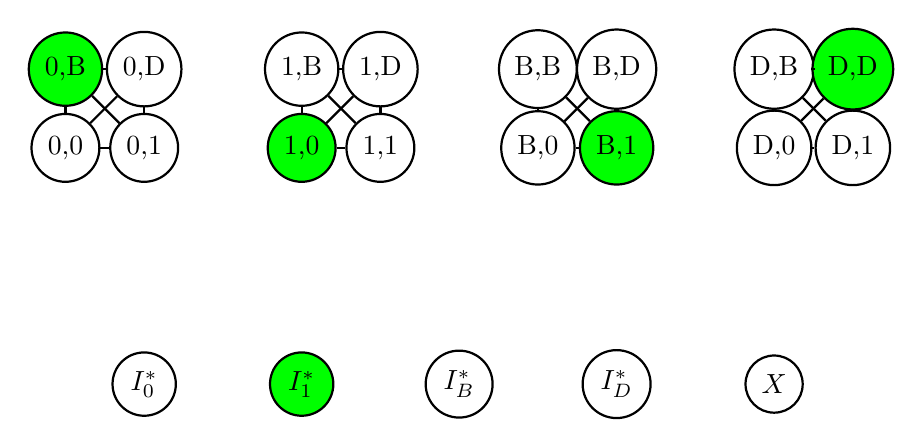
\begin{tikzpicture}
\begin{scope}[every node/.style={circle,thick,draw}]
\node (0) at (0,0)  {0,0}; 
\node (1) at (1,0)  {0,1}; 
\node (2)[fill=green] at (0,1)  {0,B}; 
\node (3) at (1,1)  {0,D}; 

\draw[thick, black] (0) -- (1); 
\draw[thick, black] (0) -- (2); 
\draw[thick, black] (0) -- (3); 
\draw[thick, black] (1) -- (2); 
\draw[thick, black] (1) -- (3); 
\draw[thick, black] (2) -- (3); 

\node (4)[fill=green] at (3,0)  {1,0}; 
\node (5) at (4,0)  {1,1}; 
\node (6) at (3,1)  {1,B}; 
\node (7) at (4,1)  {1,D}; 

\draw[thick, black] (4) -- (5); 
\draw[thick, black] (4) -- (6); 
\draw[thick, black] (4) -- (7); 
\draw[thick, black] (5) -- (6); 
\draw[thick, black] (5) -- (7); 
\draw[thick, black] (6) -- (7); 

\node (8) at (6,0)  {B,0}; 
\node (9)[fill=green] at (7,0)  {B,1}; 
\node (10) at (6,1)  {B,B}; 
\node (11) at (7,1)  {B,D}; 

\draw[thick, black] (8) -- (9); 
\draw[thick, black] (8) -- (10); 
\draw[thick, black] (8) -- (11); 
\draw[thick, black] (9) -- (10); 
\draw[thick, black] (9) -- (11); 
\draw[thick, black] (10) -- (11); 


\node (12) at (9,0)  {D,0}; 
\node (13) at (10,0)  {D,1}; 
\node (14) at (9,1)  {D,B}; 
\node (15)[fill=green] at (10,1)  {D,D}; 

\draw[thick, black] (12) -- (13); 
\draw[thick, black] (12) -- (14); 
\draw[thick, black] (12) -- (15); 
\draw[thick, black] (13) -- (14); 
\draw[thick, black] (13) -- (15); 
\draw[thick, black] (14) -- (15); 


\node (16) at (1,-3)  {$I_0^*$}; 
\node (17)[fill=green] at (3,-3)  {$I_1^*$}; 
\node (18) at (5,-3)  {$I_B^*$}; 
\node (19) at (7,-3)  {$I_D^*$}; 
\node (20) at (9, -3) {$X$}; 

\end{scope}
\end{tikzpicture}
\caption{s=5, g=5 from s=5, g=4}
\end{figure}



\section{Alternative: Constructing $g=s$ with perfect difference sets}
\emph{Though it will be shown equivalent to the last construction, we can use another concept to build these graphs: perfect difference sets.  Notably, these are proven to exist for $g=p^k$ by Singer. TODO Cite}




\begin{figure}[!htb]
\centering
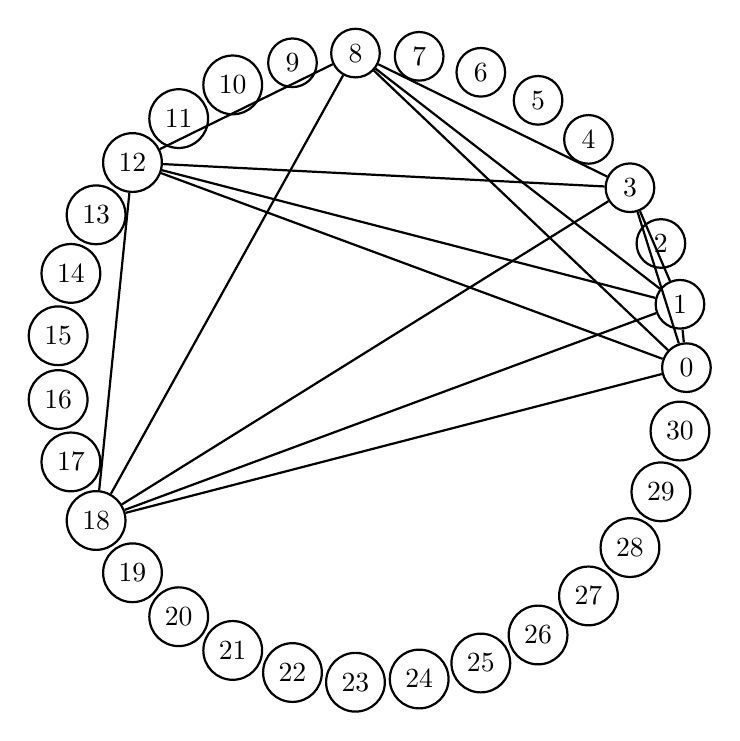
\begin{tikzpicture}
\begin{scope}[every node/.style={circle,thick,draw}]
\node (0) at (4,0) {0};
\node (1) at (3.918,0.805) {1};
\node (2) at (3.676,1.577) {2};
\node (3) at (3.283,2.285) {3};
\node (4) at (2.756,2.899) {4};
\node (5) at (2.116,3.395) {5};
\node (6) at (1.389,3.751) {6};
\node (7) at (0.606,3.954) {7};
\node (8) at (-0.203,3.995) {8};
\node (9) at (-1.003,3.872) {9};
\node (10) at (-1.762,3.591) {10};
\node (11) at (-2.448,3.163) {11};
\node (12) at (-3.035,2.605) {12};
\node (13) at (-3.497,1.941) {13};
\node (14) at (-3.817,1.197) {14};
\node (15) at (-3.979,0.405) {15};
\node (16) at (-3.979,-0.405) {16};
\node (17) at (-3.817,-1.197) {17};
\node (18) at (-3.497,-1.941) {18};
\node (19) at (-3.035,-2.605) {19};
\node (20) at (-2.448,-3.163) {20};
\node (21) at (-1.762,-3.591) {21};
\node (22) at (-1.003,-3.872) {22};
\node (23) at (-0.203,-3.995) {23};
\node (24) at (0.606,-3.954) {24};
\node (25) at (1.389,-3.751) {25};
\node (26) at (2.116,-3.395) {26};
\node (27) at (2.756,-2.899) {27};
\node (28) at (3.283,-2.285) {28};
\node (29) at (3.676,-1.577) {29};
\node (30) at (3.918,-0.805) {30};
 
  
  
\draw[thick, black] (0) -- (1); 
\draw[thick, black] (0) -- (3); 
\draw[thick, black] (0) -- (8); 
\draw[thick, black] (0) -- (12); 
\draw[thick, black] (0) -- (18); 

\draw[thick, black] (1) -- (3); 
\draw[thick, black] (1) -- (8); 
\draw[thick, black] (1) -- (12); 
\draw[thick, black] (1) -- (18); 

\draw[thick, black] (3) -- (8); 
\draw[thick, black] (3) -- (12); 
\draw[thick, black] (3) -- (18); 

\draw[thick, black] (8) -- (12); 
\draw[thick, black] (8) -- (18); 

\draw[thick, black] (12) -- (18); 


\end{scope}
,
\end{tikzpicture}
\label{fig:node5}
\caption{perfect Set difference on g=6, s=6, n=m=31}
\end{figure}




\section{Interlude: Graph Equivalence up to relabeling}

\emph{proving all $g=s$ graph colorings are the same up to relabeling.  This means that the  graphs constructed in sections X and Y are the same.}


Fig: 5 nodes each with four neighbors



\section{Constructing $g=s-1$ from the previous}

\emph{Removing one clique and all edges should suffice.}

Todo: are these all the same, looking at complement.color graph $g-1$ cliques left behind?



\section{Considering wider $g | s$ and $g | s-1$: Inception}

Rule: $g=3, s=4, n=9, m=12$

Note that since $81 = 3^4, 3 \in \mathbb{P}$, $K_{81}$ can be partitioned into 9-cliques (complete graphs of size $K_9$).  Because we can recursively construct $K_9$s from the rule below (or ``incept'' the graph), we can turn the graph $n=81, s=10, g=9, m=90$ into one of $n=81, s=40, g=3, m=1080$, in which every node still has a uniform number of attached colors, and every color has the same number of node members.  This graph has not been attempted.

\emph{Figure: s=4, g=3 has 9 nodes.  S=g=9 has 9-cliques which could be broken down }

Note: You can take the s=7, g=3, n=15, m=35 and change the n, n+5, n+10 triangles into unique colors for s=8, m=45, n=15 and g in {2,3} for example.  


\section{Considering wider $g|s$: Kirkman's schoolgirl problem}

NOTE: We have the rotator of size $g$ iff $g | s-1$, since $gk = s - 1 \Rightarrow s = gk+1 \Rightarrow m = \frac{gk+1}{s}(sg-s+1).$  This means ( I think ) that there are $k(sg-s+1)$ cliques, or $k$ rooted at each node, plus $\frac{sg-s+1}{g}$ other rotator cliques, being $s - \frac{s-1}g$ of size $g$ that are like the island triangles





\begin{figure}[!htb]
\centering
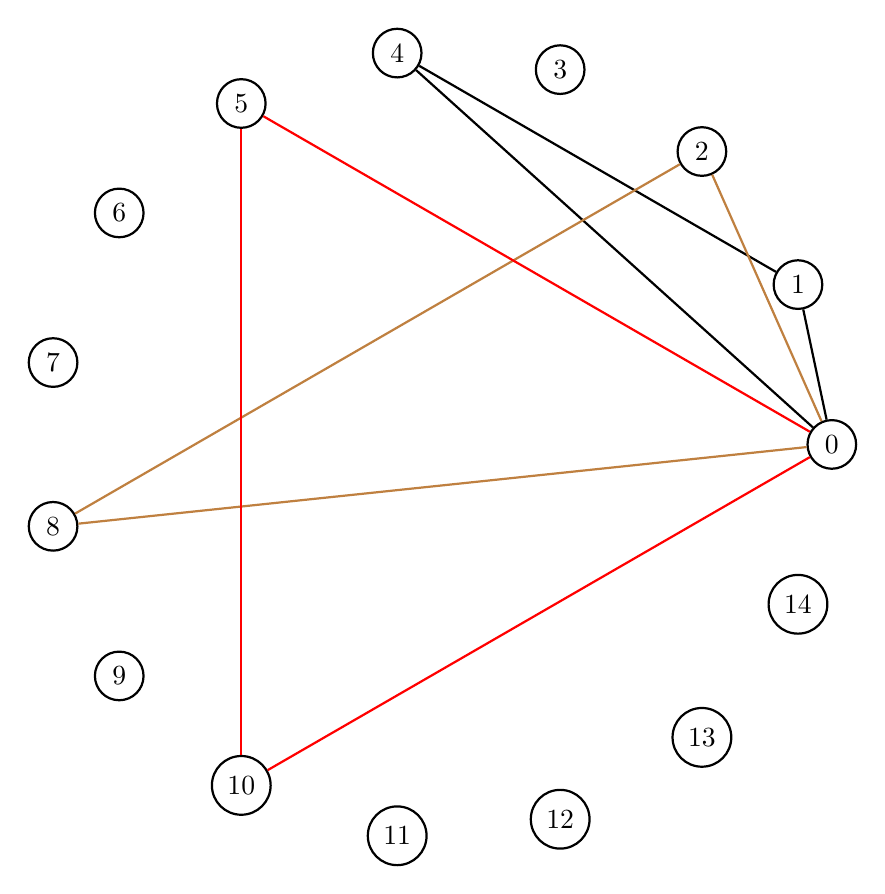
\begin{tikzpicture}
\begin{scope}[every node/.style={circle,thick,draw}]
\node (0) at (5.0, 0.0)  {0}; 
\node (1) at (4.57, 2.03) {1}; 
\node (2) at  (3.35, 3.72) {2}; 
\node (3) at  (1.55, 4.76) {3}; 
\node (4) at  (-0.52, 4.97) {4}; 
\node (5) at  (-2.5, 4.33) {5}; 
\node (6) at  (-4.05, 2.94) {6}; 
\node (7) at  (-4.89, 1.04) {7}; 
\node (8) at  (-4.89, -1.04) {8}; 
\node (9) at  (-4.05, -2.94) {9}; 
\node (10) at  (-2.5, -4.33) {10}; 
\node (11) at  (-0.52, -4.97) {11}; 
\node (12) at  (1.55, -4.76) {12}; 
\node (13) at  (3.35, -3.72) {13}; 
\node (14) at  (4.57, -2.03) {14}; 
  
\draw[thick, black] (0) -- (1); 
\draw[thick, black] (1) -- (4); 
\draw[thick, black] (0) -- (4); 

\draw[thick, brown] (0) -- (2); 
\draw[thick, brown] (2) -- (8); 
\draw[thick, brown] (0) -- (8); 

\draw[thick, red] (0) -- (5); 
\draw[thick, red] (5) -- (10); 
\draw[thick, red] (0) -- (10); 
\end{scope}
,
\end{tikzpicture}
\label{fig:s7g3}
\caption{s=7, g=3, n=15, m=35, node 0 adjacencies.  Rule: (i, i+5, i+10) x 3, (i, i+1, i+4) and (i, i+2, i+8)}
\end{figure}


ANOTHER ONE



\begin{figure}[!htb]
\centering
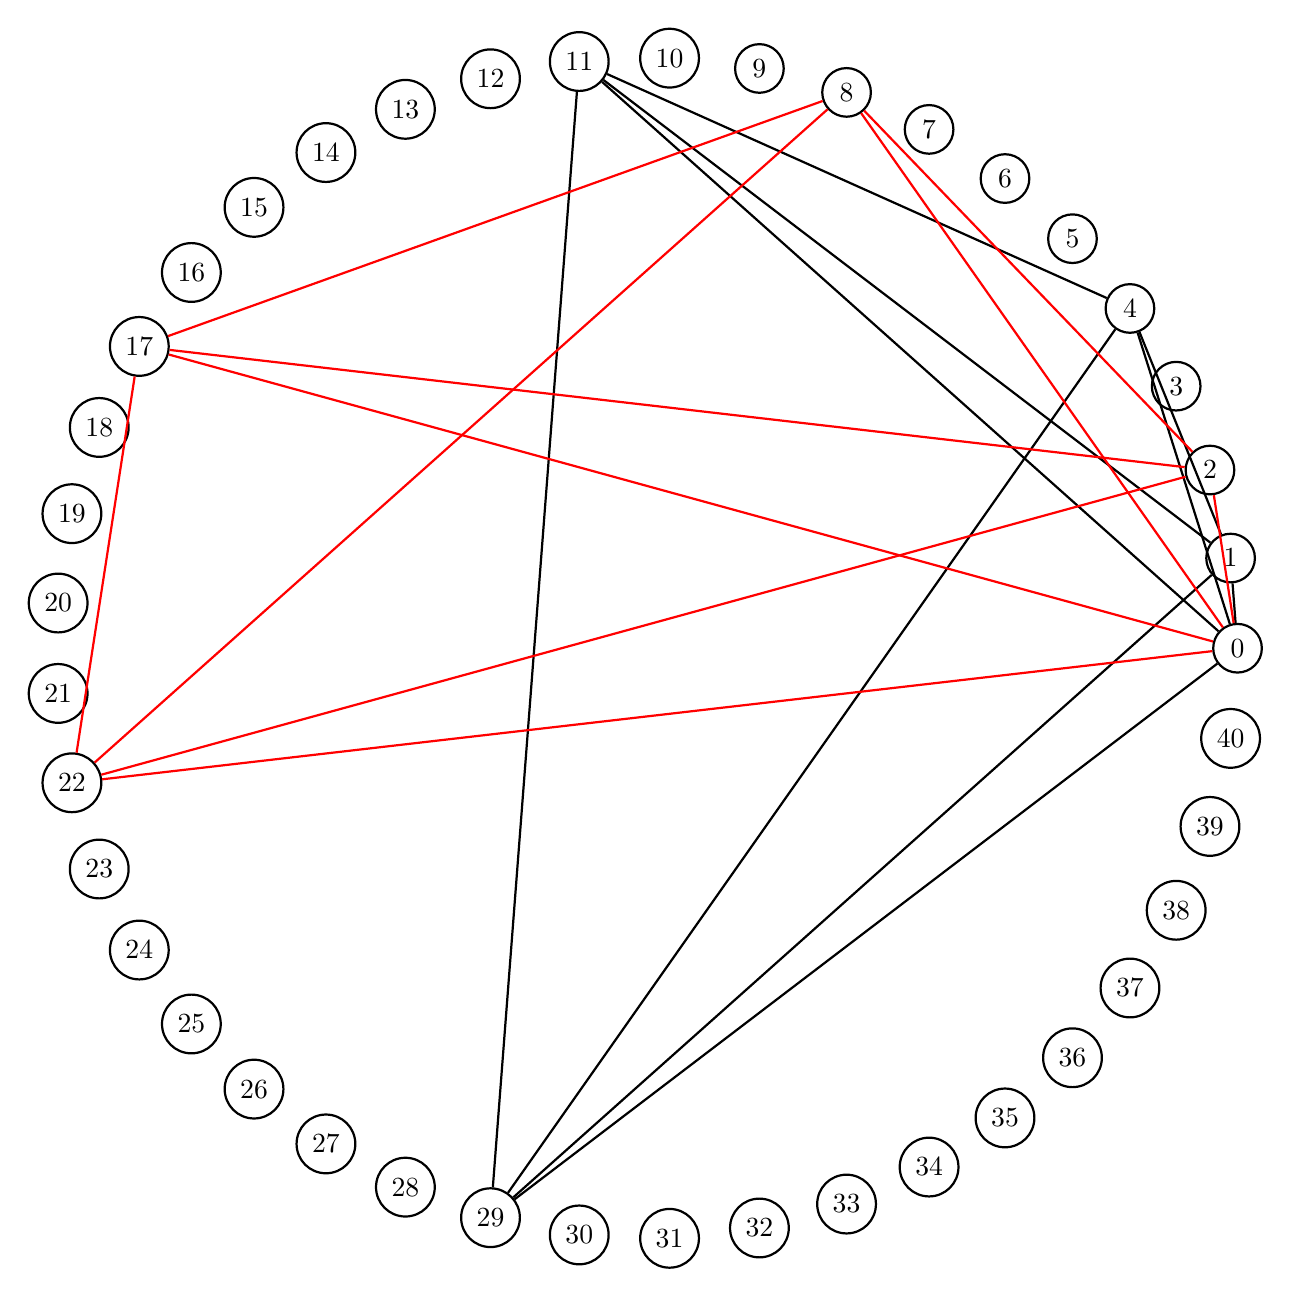
\begin{tikzpicture}
\begin{scope}[every node/.style={circle,thick,draw}]
\node (0) at (7.5,0) {0};
\node (1) at (7.412,1.145) {1};
\node (2) at (7.15,2.263) {2};
\node (3) at (6.721,3.328) {3};
\node (4) at (6.134,4.315) {4};
\node (5) at (5.404,5.201) {5};
\node (6) at (4.547,5.965) {6};
\node (7) at (3.583,6.589) {7};
\node (8) at (2.535,7.059) {8};
\node (9) at (1.428,7.363) {9};
\node (10) at (0.287,7.494) {10};
\node (11) at (-0.86,7.451) {11};
\node (12) at (-1.987,7.232) {12};
\node (13) at (-3.068,6.844) {13};
\node (14) at (-4.077,6.295) {14};
\node (15) at (-4.99,5.599) {15};
\node (16) at (-5.786,4.772) {16};
\node (17) at (-6.447,3.833) {17};
\node (18) at (-6.956,2.804) {18};
\node (19) at (-7.303,1.709) {19};
\node (20) at (-7.478,0.574) {20};
\node (21) at (-7.478,-0.574) {21};
\node (22) at (-7.303,-1.709) {22};
\node (23) at (-6.956,-2.804) {23};
\node (24) at (-6.447,-3.833) {24};
\node (25) at (-5.786,-4.772) {25};
\node (26) at (-4.99,-5.599) {26};
\node (27) at (-4.077,-6.295) {27};
\node (28) at (-3.068,-6.844) {28};
\node (29) at (-1.987,-7.232) {29};
\node (30) at (-0.86,-7.451) {30};
\node (31) at (0.287,-7.494) {31};
\node (32) at (1.428,-7.363) {32};
\node (33) at (2.535,-7.059) {33};
\node (34) at (3.583,-6.589) {34};
\node (35) at (4.547,-5.965) {35};
\node (36) at (5.404,-5.201) {36};
\node (37) at (6.134,-4.315) {37};
\node (38) at (6.721,-3.328) {38};
\node (39) at (7.15,-2.263) {39};
\node (40) at (7.412,-1.145) {40};
 
 (((0 1 4 11 29) (0 2 8 17 22)))
  
\draw[thick, black] (0) -- (1); 
\draw[thick, black] (0) -- (4); 
\draw[thick, black] (0) -- (11); 
\draw[thick, black] (0) -- (29); 

\draw[thick, black] (1) -- (4); 
\draw[thick, black] (1) -- (11); 
\draw[thick, black] (1) -- (29); 

\draw[thick, black] (4) -- (11); 
\draw[thick, black] (4) -- (29); 

\draw[thick, black] (11) -- (29); 


\draw[thick, red] (0) -- (2); 
\draw[thick, red] (0) -- (8); 
\draw[thick, red] (0) -- (17); 
\draw[thick, red] (0) -- (22); 

\draw[thick, red] (2) -- (8); 
\draw[thick, red] (2) -- (17); 
\draw[thick, red] (2) -- (22); 

\draw[thick, red] (8) -- (17); 
\draw[thick, red] (8) -- (22); 

\draw[thick, red] (17) -- (22); 


\end{scope}
,
\end{tikzpicture}
\label{fig:node5}
\caption{Perfect Difference Set on s=10, g=5, n=41, m=82: (0 1 4 11 29), (0 2 8 17 22)}
\end{figure}





\section{Nonuniform g: deletion and partial inception}



\section{Another question}

\emph{Can it be true that  $g | s(s-1)$  but not true that $g | s$ or $g | s-1$?}|


\section{THIS IS THE END}



\section{Boneyard: Some examples with $g=3$}


\begin{itemize}

\item Rule: $g=3, s=3, n=7, m=7: (0,1,3)$
\item Rule: $g=3, s=4, n = 9, m = 12: (0,3,6) \cdot 3, (0,1,2) \cdot 3, (0,4,8) \cdot 3, (0, 5,7) \cdot 3$ (this is 3 separate $K_3$, then circuit inc 0, inc1, inc 2)
\item Rule: Another example:$ g=3, s=6, n=13, m=26$.  3-graphs are at $(i, i+2, i+8)$ and $(i, i+1, i+4)$, addition being $\mod 13$..  NOTE: Is this a subset of $s=6, g=6$?
\item Rule: $g=3, s=7, n=15, m=35, (i, i+5, i+10) \cdot 3, (i, i+1, i+4), (i, i+2, i+8)$
\item Rule: $g=3, s=9, n=19, m=57: (0,1,6), (0,2,10), (0,3,7)$
\item Rule: $g=3, s=10, n=21, m=70: (0,7,14) \cdot 3, (0,2,10), (0,1,5), (0,3,9)$
\item Rule: $s=g=4, n=m=13: (0, 1, 3, 9)$
\item Rule: $(0,1,4,14,16) on s=g=5, n=21$
\item Rule: $s=g=6, n=m=31: (0, 1, 3, 8, 12, 18)$
\item NONE on $s=7=g$
\item Rule: $s=g=8, n=m=57 - (0,1, 3, 13, 32, 36, 43, 52)$
\item Rule: $s=g=9, n=m=73 - (0,1, 3, 7, 15, 31, 36, 54, 63)$  ; NOTE - these are all $2^{n-1}$ for a bit	
\item Rule: $s=g=10, n=m=91 - (0, 1, 3, 9, 27, 49, 56, 61, 77, 81)$
\item NONE on $s=g=11$
\item Rule: $g=s=12, m=n=133 - (0 1, 3, 12, 20, 34, 38, 81, 88, 94, 104, 109)$
\item NOTE All (g, s=g+1) don't seem to work with the rotators
\item TODO Build something for the 2-rotators
\end{itemize}






\begin{thebibliography}{9}
\bibitem{1} Singer, James. ``A THEOREM IN FINITE PROTECTIVE GEOMETRY AND SOME APPLICATIONS TO NUMBER THEORY'', 1934.  \url{https://www.ams.org/journals/tran/1938-043-03/S0002-9947-1938-1501951-4/S0002-9947-1938-1501951-4.pdf} 
\bibitem{2} ``The Mind-Bending Math Behind Spot It!, the Beloved Family Card Game'', Smithsonian Magazine.  \url{https://www.smithsonianmag.com/science-nature/math-card-game-spot-it-180970873/}
\bibitem{3} Wikipedia: {https://en.wikipedia.org/wiki/Graph\_partition}
\bibitem{4} Adleman, Leonard M. and Lenstra, Hendrik W.  ``FINDING IRREDUCIBLE POLYNOMIALS OVER FINITE FIELDS'' \url{https://www.math.leidenuniv.nl/~hwl/PUBLICATIONS/1986a/art.pdf}
\bibitem{5} Wikipedia: \url{https://en.m.wikipedia.org/wiki/Kirkman\%27s_schoolgirl_problem}
\end{thebibliography}


% ======= BONEYARD =======
% ======= BONEYARD =======
% ======= BONEYARD =======
% ======= BONEYARD =======
% ======= BONEYARD =======
% ======= BONEYARD =======
% DF NOTE: These are leftovers from the Dino Paper work, easy to pick up and use if needed.

\begin{comment}


\begin{figure}[!htb]
\centering
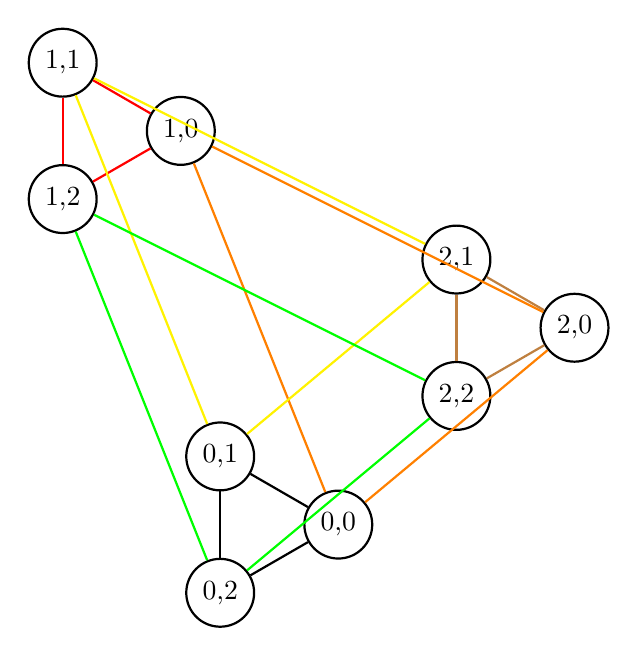
\begin{tikzpicture}
\begin{scope}[every node/.style={circle,thick,draw}]
\node (0) at (1,0)  {0,0}; 
\node (1) at (-.5, .866) {0,1}; 
\node (2) at  (-.5, -.866) {0,2}; 

\draw[thick, black] (0) -- (1); 
\draw[thick, black] (1) -- (2); 
\draw[thick, black] (0) -- (2); 

\node (3) at (-1,5)  {1,0}; 
\node (4) at (-2.5, 5.866) {1,1}; 
\node (5) at  (-2.5, 4.134) {1,2}; 

\draw[thick, red] (3) -- (4); 
\draw[thick, red] (4) -- (5); 
\draw[thick, red] (3) -- (5); 

\node (6) at (4,2.5)  {2,0}; 
\node (7) at (2.5, 3.366) {2,1}; 
\node (8) at  (2.5, 1.634) {2,2}; 

\draw[thick, brown] (6) -- (7); 
\draw[thick, brown] (7) -- (8); 
\draw[thick, brown] (6) -- (8); 

\draw[thick, orange] (0) -- (3); 
\draw[thick, orange] (3) -- (6); 
\draw[thick, orange] (0) -- (6); 


\draw[thick, yellow] (1) -- (4); 
\draw[thick, yellow] (4) -- (7); 
\draw[thick, yellow] (1) -- (7); 


\draw[thick, green] (2) -- (5); 
\draw[thick, green] (5) -- (8); 
\draw[thick, green] (2) -- (8); 





\end{scope}

\end{tikzpicture}
\label{fig:bipartite}
\caption{complete graphs with increment 0}
\end{figure}


\begin{figure}[!htb]
\centering
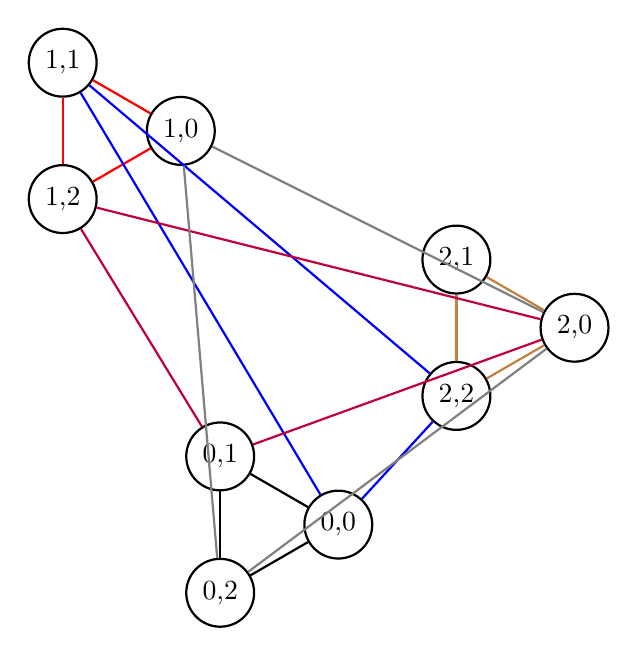
\begin{tikzpicture}
\begin{scope}[every node/.style={circle,thick,draw}]
\node (0) at (1,0)  {0,0}; 
\node (1) at (-.5, .866) {0,1}; 
\node (2) at  (-.5, -.866) {0,2}; 

\draw[thick, black] (0) -- (1); 
\draw[thick, black] (1) -- (2); 
\draw[thick, black] (0) -- (2); 

\node (3) at (-1,5)  {1,0}; 
\node (4) at (-2.5, 5.866) {1,1}; 
\node (5) at  (-2.5, 4.134) {1,2}; 

\draw[thick, red] (3) -- (4); 
\draw[thick, red] (4) -- (5); 
\draw[thick, red] (3) -- (5); 

\node (6) at (4,2.5)  {2,0}; 
\node (7) at (2.5, 3.366) {2,1}; 
\node (8) at  (2.5, 1.634) {2,2}; 

\draw[thick, brown] (6) -- (7); 
\draw[thick, brown] (7) -- (8); 
\draw[thick, brown] (6) -- (8); 

\draw[thick, blue] (0) -- (4); 
\draw[thick, blue] (4) -- (8); 
\draw[thick, blue] (0) -- (8); 


\draw[thick, purple] (1) -- (5); 
\draw[thick, purple] (5) -- (6); 
\draw[thick, purple] (1) -- (6); 


\draw[thick, gray] (2) -- (3); 
\draw[thick, gray] (3) -- (6); 
\draw[thick, gray] (2) -- (6); 
\end{scope}

\end{tikzpicture}
\label{fig:bipartite}
\caption{complete graphs with increment 1}
\end{figure}


\begin{figure}[!htb]
\centering
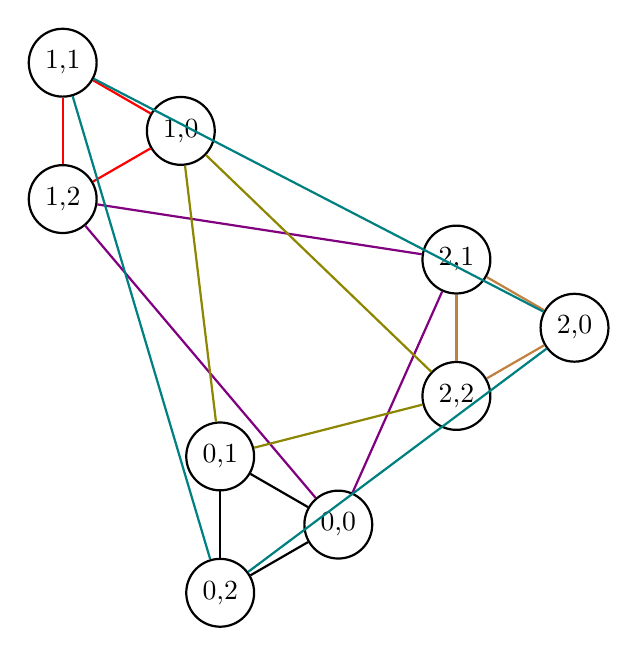
\begin{tikzpicture}
\begin{scope}[every node/.style={circle,thick,draw}]
\node (0) at (1,0)  {0,0}; 
\node (1) at (-.5, .866) {0,1}; 
\node (2) at  (-.5, -.866) {0,2}; 

\draw[thick, black] (0) -- (1); 
\draw[thick, black] (1) -- (2); 
\draw[thick, black] (0) -- (2); 

\node (3) at (-1,5)  {1,0}; 
\node (4) at (-2.5, 5.866) {1,1}; 
\node (5) at  (-2.5, 4.134) {1,2}; 

\draw[thick, red] (3) -- (4); 
\draw[thick, red] (4) -- (5); 
\draw[thick, red] (3) -- (5); 

\node (6) at (4,2.5)  {2,0}; 
\node (7) at (2.5, 3.366) {2,1}; 
\node (8) at  (2.5, 1.634) {2,2}; 

\draw[thick, brown] (6) -- (7); 
\draw[thick, brown] (7) -- (8); 
\draw[thick, brown] (6) -- (8); 

\draw[thick, violet] (0) -- (5); 
\draw[thick, violet] (5) -- (7); 
\draw[thick, violet] (0) -- (7); 


\draw[thick, olive] (1) -- (3); 
\draw[thick, olive] (3) -- (8); 
\draw[thick, olive] (1) -- (8); 


\draw[thick, teal] (2) -- (4); 
\draw[thick, teal] (4) -- (6); 
\draw[thick, teal] (2) -- (6); 


\end{scope}

\end{tikzpicture}
\label{fig:bipartite}
\caption{complete graphs with increment 2}
\end{figure}



\begin{figure}[!htb]
\centering
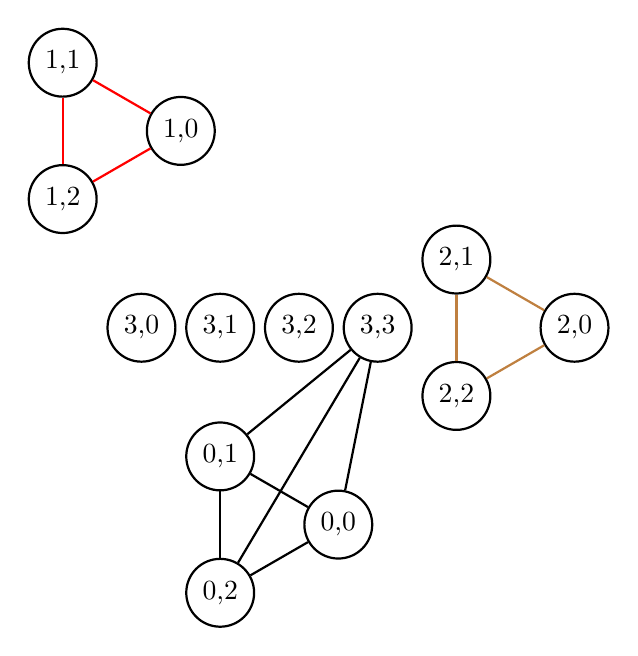
\begin{tikzpicture}
\begin{scope}[every node/.style={circle,thick,draw}]
\node (0) at (1,0)  {0,0}; 
\node (1) at (-.5, .866) {0,1}; 
\node (2) at  (-.5, -.866) {0,2}; 

\draw[thick, black] (0) -- (1); 
\draw[thick, black] (1) -- (2); 
\draw[thick, black] (0) -- (2); 

\node (3) at (-1,5)  {1,0}; 
\node (4) at (-2.5, 5.866) {1,1}; 
\node (5) at  (-2.5, 4.134) {1,2}; 

\draw[thick, red] (3) -- (4); 
\draw[thick, red] (4) -- (5); 
\draw[thick, red] (3) -- (5); 

\node (6) at (4,2.5)  {2,0}; 
\node (7) at (2.5, 3.366) {2,1}; 
\node (8) at  (2.5, 1.634) {2,2}; 

\draw[thick, brown] (6) -- (7); 
\draw[thick, brown] (7) -- (8); 
\draw[thick, brown] (6) -- (8); 


\node (9) at (-1.5, 2.5) {3,0};
\node (10) at (-.5, 2.5) {3,1};
\node (11) at (.5, 2.5) {3,2};
\node (12) at (1.50, 2.5) {3,3};

\draw[thick, black] (12) -- (0); 
\draw[thick, black] (12) -- (1); 
\draw[thick, black] (12) -- (2); 

\end{scope}
\end{tikzpicture}
\label{fig:bipartite}
\caption{$s=4, g=4, n=13, m=13$: adding to original cliques - 3,3 adds to each original}
\end{figure}

\begin{figure}[!htb]
\centering
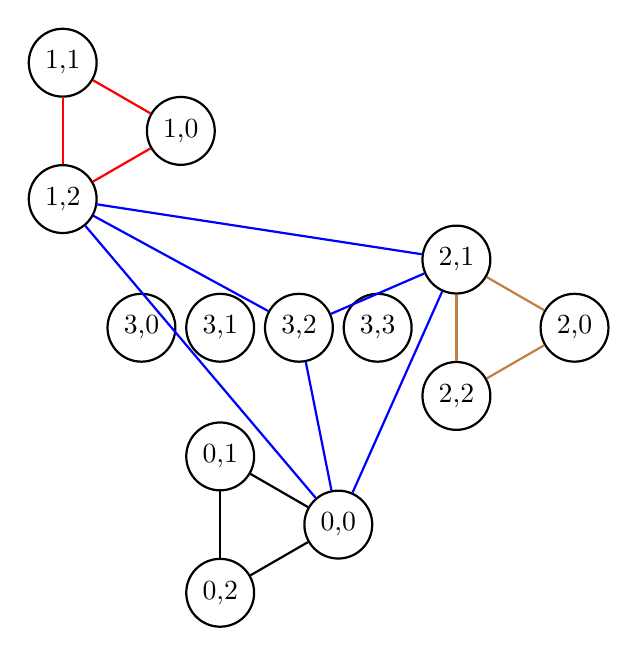
\begin{tikzpicture}
\begin{scope}[every node/.style={circle,thick,draw}]
\node (0) at (1,0)  {0,0}; 
\node (1) at (-.5, .866) {0,1}; 
\node (2) at  (-.5, -.866) {0,2}; 

\draw[thick, black] (0) -- (1); 
\draw[thick, black] (1) -- (2); 
\draw[thick, black] (0) -- (2); 

\node (3) at (-1,5)  {1,0}; 
\node (4) at (-2.5, 5.866) {1,1}; 
\node (5) at  (-2.5, 4.134) {1,2}; 

\draw[thick, red] (3) -- (4); 
\draw[thick, red] (4) -- (5); 
\draw[thick, red] (3) -- (5); 

\node (6) at (4,2.5)  {2,0}; 
\node (7) at (2.5, 3.366) {2,1}; 
\node (8) at  (2.5, 1.634) {2,2}; 

\draw[thick, brown] (6) -- (7); 
\draw[thick, brown] (7) -- (8); 
\draw[thick, brown] (6) -- (8); 


\node (9) at (-1.5, 2.5) {3,0};
\node (10) at (-.5, 2.5) {3,1};
\node (11) at (.5, 2.5) {3,2};
\node (12) at (1.50, 2.5) {3,3};

\draw[thick, blue] (0) -- (5); 
\draw[thick, blue] (5) -- (7); 
\draw[thick, blue] (0) -- (7); 


\draw[thick, blue] (11) -- (0); 
\draw[thick, blue] (11) -- (5); 
\draw[thick, blue] (11) -- (7); 


\end{scope}
\end{tikzpicture}
\label{fig:bipartite}
\caption{adding to increment cliques  - 3,2 adds to all 2 increment cliques}
\end{figure}
\end{comment} 

\end{document}


